\subsubsection{An\'alise Explorat\'oria dos dados (EDA)}

A partir do passo \ref{etp:1}, foi realizado o EDA (Exploratory Data Analysis) para processar os dados obtidos até o momento. O EDA permite responder às questões de pesquisa levantadas. Conforme mencionado por \citeonline{Yu2016}, na era dos grandes dados, é desafiador descobrir as regras, modelos analíticos e hipóteses por trás dos volumes massivos de dados caóticos, não estruturados e multimídia coletados por meio de vários canais. A análise exploratória de dados foi promovida por John Tukey como uma abordagem para explorar os dados, resumir suas principais características e formular hipóteses que possam direcionar a coleta adicional de dados e experimentos. No contexto de grandes análises de dados, várias técnicas de EDA têm sido adotadas.

Ao analisar a pergunta \ref{q1}, que relaciona a demanda com a variável prevista e a pressão para a variável PT01, pode-se observar na Figura \ref{fig:person} que ambas as variáveis apresentam uma correlação quase perfeita, com um coeficiente de correlação de Pearson ($r$) igual a 1. Portanto, para responder a essa pergunta, basta observar a correlação de Pearson na Figura \ref{fig:person}.

Para responder à pergunta \ref{q2}, é criada uma tabela para fornecer uma resposta mais completa.


\begin{table}[H]
	\centering
	\caption{Descrição estatística dos dados com o filtro aplicado das 18h às 21h}\label{tb:est}
	\begin{tabular}{@{}cccccccccc@{}}
		\toprule
		\textbf{18 a 21h}  & \textbf{B1} & \textbf{B2} & \textbf{B3} & \textbf{LT01} & \textbf{FT01} & \textbf{FT02} & \textbf{FT03} & \textbf{PT01} & \textbf{PT02} \\ \midrule
		\textbf{Contagem} & 366         & 366         & 366         & 366           & 366           & 366           & 366           & 366           & 366           \\
		\textbf{Média}    & 43,87       & 22,26       & 8,70        & 3,34          & 164,83        & 133,08        & 102,01        & 4,23          & 17,29         \\
		\textbf{STD}      & 23,22       & 18,47       & 17,81       & 0,69          & 114,60        & 67,99         & 47,55         & 0,81          & 8,59          \\
		\textbf{Min}      & 0           & 0           & 0           & 0,99          & 0,07          & 0             & 0             & 1,88          & 0             \\
		\textbf{25\%}     & 37,93       & 0           & 0           & 2,87          & 64,31         & 131,06        & 107,92        & 3,69          & 16,77         \\
		\textbf{50\%}     & 57,99       & 30,92       & 0           & 3,41          & 201,37        & 146,17        & 121,40        & 4,22          & 22,46         \\
		\textbf{75\%}     & 57,99       & 37,25       & 0           & 3,86          & 268,61        & 158,71        & 127,07        & 4,85          & 22,52         \\
		\textbf{Max}      & 59,99       & 57,33       & 53,74       & 4,40          & 379,20        & 285,56        & 170,56        & 5,66          & 24,23         \\ \bottomrule
	\end{tabular}
	
	Fonte: Elaboração própria a partir de dados da SANEPAR (2018 a 2020)
\end{table}

Na Tabela \ref{tb:est}, o desvio padrão é representado pela sigla STD, que corresponde à expressão em inglês "standard deviation". Além disso, em resposta à pergunta \ref{q2}, é importante mencionar que, assim como em qualquer empresa de tratamento de água, é utilizado um mecanismo de acionamento automático chamado "trava de segurança" para evitar que o nível do tanque chegue a zero e haja falta de água nos locais abastecidos por esse tanque. O nível mínimo que o tanque pode alcançar é de $1.459 m^3$ (equivalente a 1459 litros). As bombas são ativadas em sua potência máxima para evitar que sejam acionadas quando o nível do tanque estiver fora da faixa de $[3.843, 4.256]\ m^3$. No entanto, a bomba 1 ainda estaria operando para completar o nível do tanque caso ele esteja dentro dessa faixa.

Em situações de demanda de pico, uma abordagem ideal, embora não necessariamente a mais econômica, seria ter um tanque de reserva adicional e instalar uma tubulação que os conecte. Durante o dia, ambos os tanques seriam abastecidos e, à noite, por meio da ação da gravidade, eles manteriam o mesmo nível até que o consumo atinja um ponto em que as bombas sejam acionadas. Essa estratégia permite um abastecimento contínuo e eficiente de água.



%\begin{figure}[H]
%	\centering
%	\caption{Solução para o acionamento das bombas}
%	\label{fig:esquema}
%	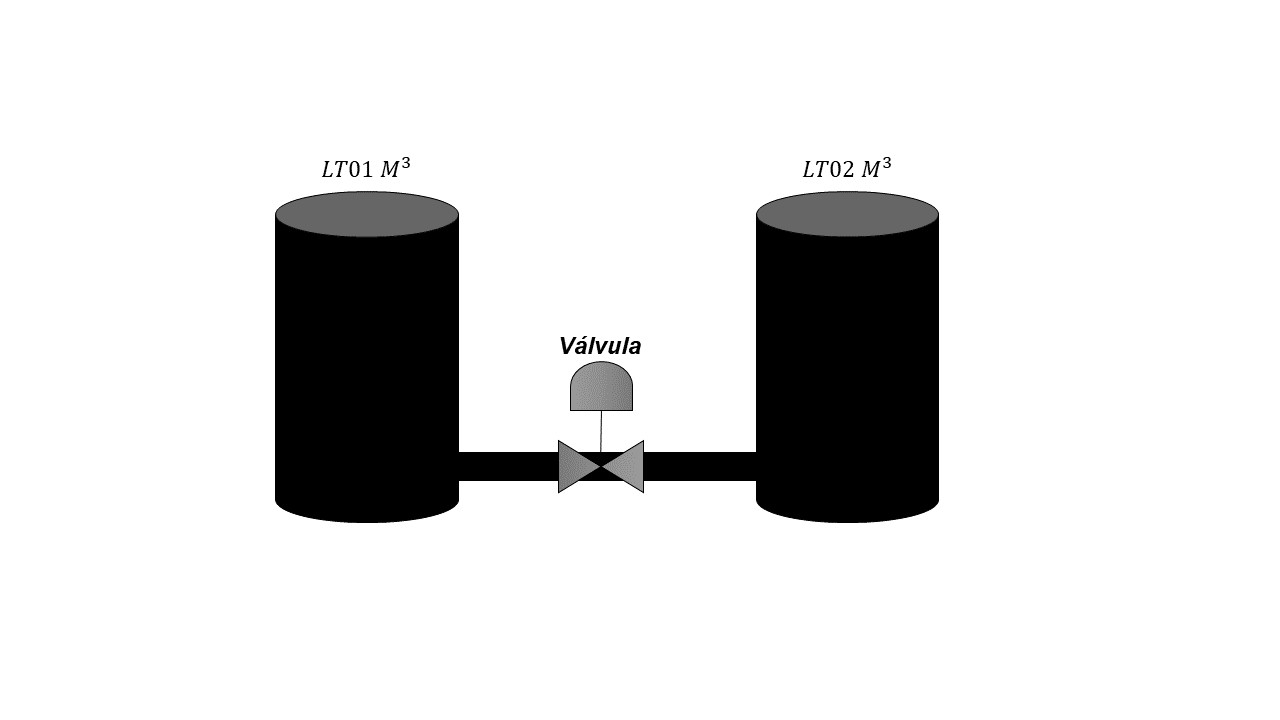
\includegraphics[width=1\linewidth]{Resultados/Figuras/esquema}
%	Fonte: Elaboração própria 
%\end{figure}
%
%Na Figura \ref{fig:esquema} um esquema prático para evitar a escassez de água e o consumo em horários de pico. Este é um esquema muito simples de como a hora do dia pode ser melhorada para o armazenamento de água.

Na pergunta \ref{q3}, observa-se que o tanque tem uma capacidade máxima de $4,256 m^3$, o que equivale a $4.256$ litros. Para atender a essa demanda e manter o tanque quase cheio ou sempre cheio, é necessário que o fluxo de entrada esteja na faixa de $[238, 302] \ m^3/h$, o fluxo de gravidade esteja entre $[126, 182] \ m^3/h$, o fluxo de retorno esteja entre $[110, 144] \ m^3/h$, a pressão de sucção esteja entre $[1.92, 4.24] \ mca$ e a pressão de retorno esteja entre $[21, 24] \ mca$.

Para responder à pergunta \ref{q4}, o ponto de equilíbrio, onde as bombas não precisam ser acionadas, ocorre quando o fluxo de FT01 é de $211 \ m^3/h$, FT02 é de $114 \ m^3/h$, FT03 é de $100 \ m^3/h$ e o nível do tanque está em $3.545 \ m^3$.
No que diz respeito à pergunta \ref{q5}\ref{q5:a}, o nível do tanque deve ser de $4,00 \ m^3$ para evitar o funcionamento das bombas durante as horas de pico.